\documentclass[12pt]{article}
\usepackage{geometry}                % See geometry.pdf to learn the layout options. There are lots.
\geometry{letterpaper}                   % ... or a4paper or a5paper or ... 
%\geometry{landscape}                % Activate for for rotated page geometry
%\usepackage[parfill]{parskip}    % Activate to begin paragraphs with an empty line rather than an indent
\usepackage{graphicx}
\usepackage{amssymb}



\title{Analysis of loadings}
\author{Wesley Brooks}
\date{}                                           % Activate to display a given date or no date

\usepackage{Sweave}
\begin{document}
\maketitle

First, we'll read in the data files.


Figure out what proportion of total storm loading is contributed by the top 10\% of storms:


The top 10\% of storms contributed 92.4\% of the storm loading at Eagle Creek, 81.3\% of the storm loading at Otter Creek, and 95.8\% of the storm loading at Joos Valley Creek.


\begin{figure}
  \begin{center}
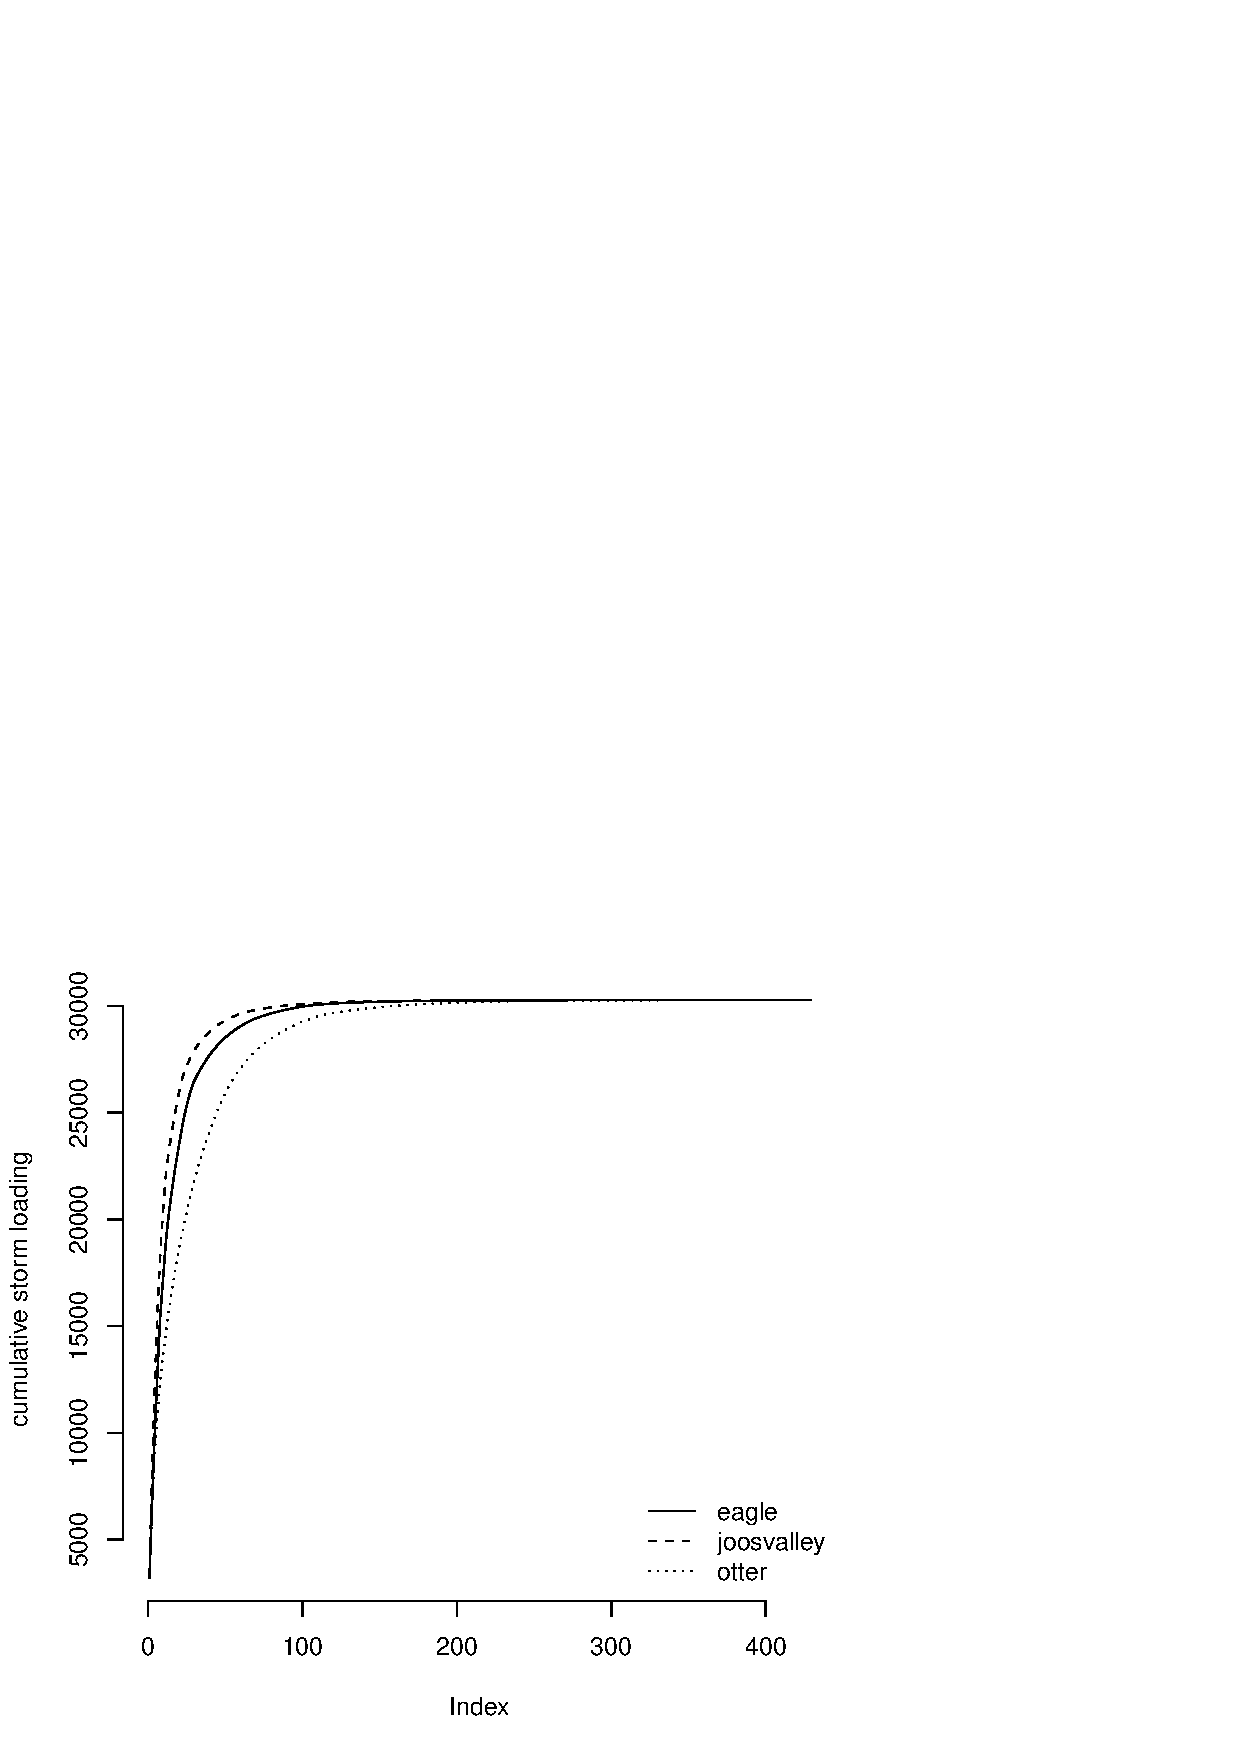
\includegraphics{loadings-figure1}
  \end{center}
  \caption{Cumulative storm loadings at the three creeks.\label{cdf}}
\end{figure}


Now we will use \verb!rpart! to make a decision tree for major events.


\begin{Schunk}
\begin{Soutput}
n= 1326 

node), split, n, deviance, yval
      * denotes terminal node

 1) root 1326 120.45850 0.101055800  
   2) pstorm_max< 66.895 1175  13.83319 0.011914890  
     4) sstorm_tot< 15.95 1143   1.99650 0.001749781 *
     5) sstorm_tot>=15.95 32   7.50000 0.375000000  
      10) stream=eagle 20   0.00000 0.000000000 *
      11) stream=joosvalley,otter 12   0.00000 1.000000000 *
   3) pstorm_max>=66.895 151  24.63576 0.794702000  
     6) pstorm_tot< 180.42 51  12.74510 0.490196100  
      12) stream=eagle 20   0.00000 0.000000000 *
      13) stream=joosvalley,otter 31   4.83871 0.806451600  
        26) stot_tot< 17.595 9   2.00000 0.333333300 *
        27) stot_tot>=17.595 22   0.00000 1.000000000 *
     7) pstorm_tot>=180.42 100   4.75000 0.950000000 *
\end{Soutput}
\end{Schunk}




\end{document}
